% Explication générale de méthodes de programmation
\section{Management du code}
\subsection{Versionnage}
Git
\subsection{Construction logicielle}
CMake
\subsubsection{Résolution de la dépendance}
Module CMake
\subsection{Tests unitaires}
CMake via Ctest
\subsection{Tests d'intégration}
CMake via Ctest
Scénario -> Test unitaire en BN
\subsection{Tests de couverture}
Lcov
\subsection{Documentation}
Doxygen + Wiki
\subsection{Repporting}
\subsection{Intégration continue}
Jenkins

\section{Développement de framework}
Cette section présente quelques techniques de programmation, idiomes et pattern qui seront utilisés de manière globale pour l'ensemble de la modélisation et de la réalisation du projet.
\subsection{Idiome NVI}
\subsubsection{Présentation}
L'idiome NVI, pour Non-Virtual Interface, est la réalisation en C++ du design pattern Template Method. Il possède plusieurs avantages notamment dans le développement d'un framework.\\
Il consiste à maintenir la consistance de certains comportements en un point de contrôle du code défini par le développeur. Cela permet d'une inversion de contrôle bénéfique dans de nombreux cas, dont le cas d'un framework puisqu'il déresponsabilise l'utilisateur final de certaines contraintes qui ne pourraient être exprimées que par de la documentation et dont le non respect entrainerait des comportements inattendus difficiles à localiser.\\
NVI est guidé par 4 règles décrites par Herb Sutter dans son article sur la virtualité :
\begin{itemize}
\item Prefer to make interfaces nonvirtual, using Template Method design pattern.
\item Prefer to make virtual functions private.
\item Only if derived classes need to invoke the base implementation of a virtual function, make the virtual function protected.
\item A base class destructor should be either public and virtual, or protected and nonvirtual.
\end{itemize}

\subsubsection{Exemple}
Imaginons une bibliothèque de manipulation de matrices. La bibliothèque propose une classe abstraite Matrice avec l'API globale de toute matrice. On considérera ici la calcul du déterminant. Découle de cette classe une hiérarchie de matrices pour les cas particuliers : matrice triangulaire, matrice diagonale, etc.\\

\begin{figure}[!h]\centering
    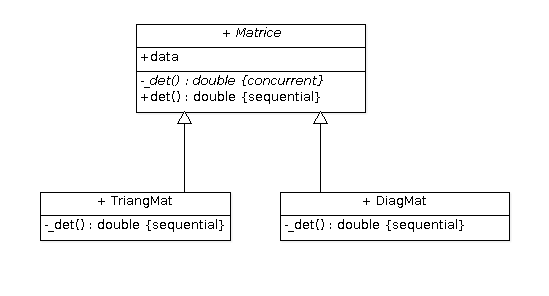
\includegraphics[scale=0.7]{images/nvi_illu.png}
    \caption{\label{nvi_uml} Illustration du NVI.}
\end{figure}

\begin{lstlisting}[label=nvi_code,caption=NVI : principe.,language=C++]
class Matrice
{
public :
    double det() const
    {
        // Pre-traitement : verification d'invariants, lock multithread, etc.
        m.lock();
        assert(data_.check_invariants() == true);
        // Appel de l'implementation
        return _det();
        // Post-traitement
        assert(data_.check_invariants() == true);
        m.unlock();
    }
    
private :
    virtual double _det() const = 0;
    
protected :
    Data data;
    mutex m;
};

class TriangMat : public Matrice
{
private :
    virtual double _det() const 
    {
        // Retourne le produit de la diagonale
    }
}

class DiagMat : public Matrice
{
private :
    virtual double _det() const 
    {
        // Retourne le produit de la diagonale
    }
}
\end{lstlisting}

Ainsi, lorsque l'utilisateur voudra ajouter une nouvelle matrice, disons de forme Hessenberg, il aura simplement à implémenter le calcul du déterminant, les invariants étant toujours vérifiés dans le code de la classe de base qui va appeler l'implémentation.\\
Il y a donc une réelle inversion de contrôle et c'est le développeur du framework qui dirige le client à l'utiliser correctement.\\\\

Nous utiliserons par la suite du projet l'idiome NVI de manière intensive pour permettre de guider le flux d'exécution.

\subsection{Paramétrage par politique}
\subsubsection{Présentation}
Le paramétrage par politique est une technique de programmation développée et démocratisée par Andrei Alexandrescu dans son livre Modern C++ Design: Generic Programming and Design Patterns Applied et dans la bibliothèque Loki dédiée à la méta-programmation en C++ dont beaucoup d'éléments ont été repris dans Boost puis dans le standard 2011.\\\\
Concrètement, il s'agit de profiter de l'héritage multiple et de la métaprogrammation pour permettre de séparer les différents comportements d'une classe ou de plusieurs classes et de créer sur mesure des comportements en combinant plusieurs politiques.

\subsubsection{Fonctionnement}
La clef d'un paramétrage par politique efficace réside dans l'analyse des différents comportements d'une classe ou d'un ensemble de classes. Imaginons que nous ayons à créer une bibliothèque de gestion de graphes. Un graphe peut être représenté sous différentes formes : matrice d'adjacence, matrice d'incidence , ou liste de successeurs. Chaque représentation à ses avantages et ses inconvénients en fonction des applications. On pourrait aisément créer 3 classes différentes mais cela ne serait pas très pertinent. On pourrait simplement templater la classe de graphe mais chaque type donnée n'a pas la même API. De plus, imaginons qu'un graphe puisse être partagé entre plusieurs thread ou non selon les applications.\\
Sans paramétrage par politique, il faudrait un nombre de classes égales au nombre de facteurs multiplié par le nombre de modes par facteur. Cela apporterait évidemment du code redondant et une maintenabilité moindre puisque dans le cas d'un paramétrage par politique on peut isoler complètement un comportement. Pour modifier l'intégralité du modèle multithread d'une application, la modification d'une seule classe de politique est nécessaire.\\\\

Chaque facteur est représenté par une classe abstraite permettant de définir l'API commune à tous les modes et qui pourra être utilisée par les classes paramétrées avec ce facteur. Les classes concrètes implémentent chacun des modes de la politique.\\
Enfin, la classe de services qui doit être paramétrée par politique va être templaté avec chacune des politique et en hériter de manière publique ou privée selon les besoins.

\subsubsection{Exemple}

\begin{figure}[!h]\centering
    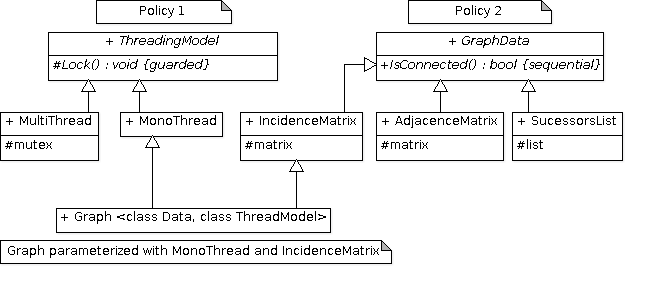
\includegraphics[scale=0.7]{images/policy_illu.png}
    \caption{\label{policy_uml} Illustration du paramétrage par politique.}
\end{figure}

On définit la première hiérarchie de classes correspondant à la première politique :
\begin{lstlisting}[label=policy_1,caption=Définition de la première politique,language=C++]
class ThreadingModel 
{
protected :
    virtual void Lock() = 0;
};

class MultiThread : public ThreadingModel
{
protected :
    virtual void Lock()
    {
        m.lock();
    }
    
    std::mutex m;
};

class MonoThread : public ThreadingModel
{
protected :
    virtual void Lock() = default
};

// ... Autres modeles ...
\end{lstlisting}

On définit la seconde politique :
\begin{lstlisting}[label=policy_2,caption=Définition de la seconde politique,language=C++]
class IncidenceMatrix : public GraphRepresentation
{
public :
    virtual bool IsConnected() const
    {
        // Determine si un graphe est connexe
    }
protected :
    std::vector<std::vector<int>> data;
};

class AdjacenceMatrix : public GraphRepresentation
{
public :
    virtual bool IsConnected() const
    {
        // Determine si un graphe est connexe
    }
protected :
    std::vector<std::vector<bool>> data;
};

//... Autres representations ...
\end{lstlisting}

On définit la classe principale de graphe et on la paramétrise à l'instanciation selon les besoins :
\begin{lstlisting}[label=policy_3,caption=Illustration de la paramétrisation,language=C++]
template <class Rep = AdjacenceMatrix, class ThreadModel = MonoThread>
class Graph : public Rep, public ThreadModel
{
public :
    bool IsConnected() const
    {
        ThreadModel::Lock();
        return Rep::IsConnected();
    }
};

using GraphInciMT = Graph<IncidenceMatrix, MultiThread>;
using GraphAdjMT = Graph<AdjacenceMatrix, MultiThread>;

// Exemples
Graph a; // Adjacence, MonoThread
GraphInciMT b; // Incidence, MultiThread
GraphAdjMT c; // Adjacence, MultiThread

\end{lstlisting}

La classe Graph fait appelle à l'aveugle à sa politique de thread ainsi qu'à sa politique de représentation. La bonne écriture d'une politique est guidée par l'API de la classe abstraite en haut de la hiérarchie mais aucune vérification de type n'est effectuée par la classe Graph. Ainsi, un utilisateur pourrait écrire sa propre politique qui ne serait pas basée sur une des classes abstraites.\\
La vérification s'effectue à la compilation en regardant les parties de l'API utilisée (ici la méthode Lock et IsConnected) ce qui est moins restrictif que le typage. On voit clairement l'avantage en terme de maintenabilité puisque la politique ThreadingModel sera surement partagée par l'ensemble des classes de l'application et ainsi, si le modèle doit évoluer, l'ensemble de la gestion multithread se trouve dans une seule classe. On isole la technologie (\verb|std::thread|, \verb|pthread|, \verb|boost::thread|, etc.) et on peut répercuter un changement dans le modèle sur l'ensemble de l'application très facilement.\\\\
La partie \verb|using| n'est pas du simple sucre synthaxique puisqu'il contribue également à la maintenabilité de l'application. L'utilisateur final utilise des types en \og{} dur \fg, sans template, ce qui permet, si le besoin s'en fait sentir, de ne changer le template qu'à un unique endroit.
